\subsection{Statistische Analyse von Höhendaten}
\usetikzlibrary{decorations.pathreplacing}
Ausserhalb der gewöhnlichen statistischen Analyse, die wir
hier als bekannt voraussetzen, führen wir hier weitere Werkzeuge
ein, die sich spezial für die Analyse rauer Oberflächen bzw. 
Gitterstrukturen als nützlich erweisen\cite{gwyddion}. Zunächst
gehen wir davon aus, dass uns die Mikroskopiedaten als 
$N \times M$ Vektorfeld vorliegen (N Zeilen und M Spalten der
Matrix der Bilddaten, ). Die tatsächliche Fläche der Daten
nennen wir nun $L_x \times L_y$, wobei 
wir ObdA nehmen nun annehmen, dass die Abstände
zwischen den Datenpunkten $\Delta$ betrage 
(siehe Abbildung~\ref{fig:stat1}). 

\begin{figure}
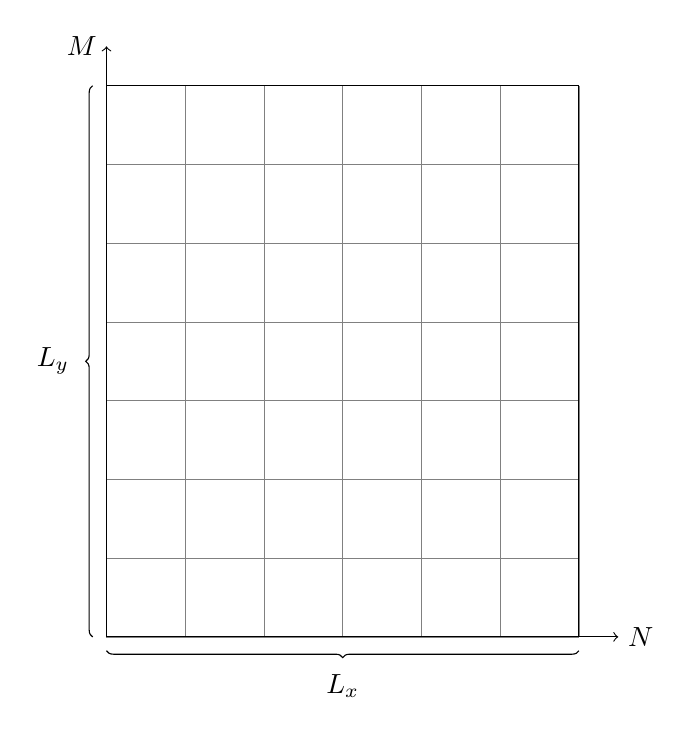
\begin{tikzpicture}
\draw[step=1cm,gray,very thin] (-1,-1) grid (5,6);
\draw  (-1,-1) -- (5,-1) -- (5,6) -- (-1,6) -- (-1,-1);
\draw [<->] (-1,6.5) node [left]{$M$} -- (-1,-1) 
-- (5.5,-1) node [right] {$N$};
\draw [decoration={brace,mirror,raise=5pt},decorate]
(-1,-1) --  node[below=10pt]{$L_x$}(5,-1); 

\draw [decoration={brace,raise=5pt},decorate]
(-1,-1) --  node[left=10pt]{$L_y$}(-1,6); 

\end{tikzpicture}
\caption{Das Vektorfeld der Mikroskopiedaten besteht aus 
$N \times M$ Höhendaten aus $\mathbb{R}$, wobei die tatsächliche 
Fläche $L_x \times L_y$ beträgt.}
\label{fig:stat1}
\end{figure}
Wir betrachten nun 
die statistischen Eigenschaften der Zufallsvariablen $\xi(x,y)$. 
Die Wahrscheinlichkeitsdichte $\rho(x,y,z)$ für eine 
bestimmte Höhe $z$ ergibt sich numerisch
durch die Extrapolation der einzelnen Datenpunkte mit der Normierung:
\begin{equation*}
\int \rho(x,y,z) dx dy dz = 1
\end{equation*}
\subsubsection{Fourier Transformationen}
Sei nun ganz allgemein die Fouriertransformation eingeführt:
\begin{align}
f(x) &= \int_{-\infty}^{\infty} F(k)\exp(2\pi i kx)dk\\
F(k) &= \mathcal{F}_x\left [f(x)\right ](k) =
\int_{-\infty}^{\infty} f(k)\exp(-2\pi i kx)dx
\end{align}
Mit den (nur den wichtigsten) Eigenschaften:
\begin{align}
&\mathcal{F}\left [a f(x) + b g(x)\right ]
    = a F(k) + b G(k) 
    &\mbox{ (Linearität) }\\
&\mathcal{F}\left [f(x) * g(x)\right ](k)
    = \mathcal{F}\left [f(x)\right ]\mathcal{F}\left [g(x)\right ]
    \! &\mbox{ (Faltungseigenschaft) }\\
&\mathcal{F}_k\left [\left | F(k) \right |^2\right ](x)
   =  \int_{-\infty}^{\infty}\bar{f}(\tau)f(\tau + x) d\tau 
   &\mbox{ (Wiener-Khinchin Theorem) }
\end{align}
In der letzten Eigenschaft
bedeutet $\bar{f}$ die komplexe Konjugation von $f$.
Die Definitionen sind nun für die x-Richtung ausgeführt worden,
sie funktionieren jedoch analog im $2D$ Fall, also mit dem Tuple
$(x,y)$. In der numerischen Analyse wird nun die ``Schnelle''
Fouriertransform (engl. \textit{Fast Fourier Transform, FFT})
berechnet. \\Da wir die Integraltransformationen
bei einem begrenzten und
nicht unendlichen Datensatz mit der
diskreten Fourier Transformation (DFT)
approximieren müssen, implizieren wir zyklische Randbedingungen:
\begin{align}
 &f(n) = \frac{1}{N}\sum_{n=0}^{N-1}{\exp(2\pi i \frac{kn}{N})f(k) }\\
 &F(k) = \sum_{n=0}^{N-1}{\exp(-2\pi i \frac{kn}{N})f(n) }
\end{align}
Da die realen Datensätze diese Bedingungen nicht aufweisen, müssen
die Ränder des Datensatzes ``unterdrückt'' bzw. transformiert
werden. Generell wird dazu eine Fensterfunktion (\textit{Window
function}) verwendet, welche mit dem Signal gefaltet wird und
somit die bei der FFT auftretenden Randeffekte zu unterdrücken 
sucht. Dabei sind verschiedene Windowfunctions denkbar, welche
über verschiedene Güten verfügen und an die Eigenschaften
des Signals angepasst werden müssen (siehe Abbildung~\ref{fig:stm2}).
\begin{figure}
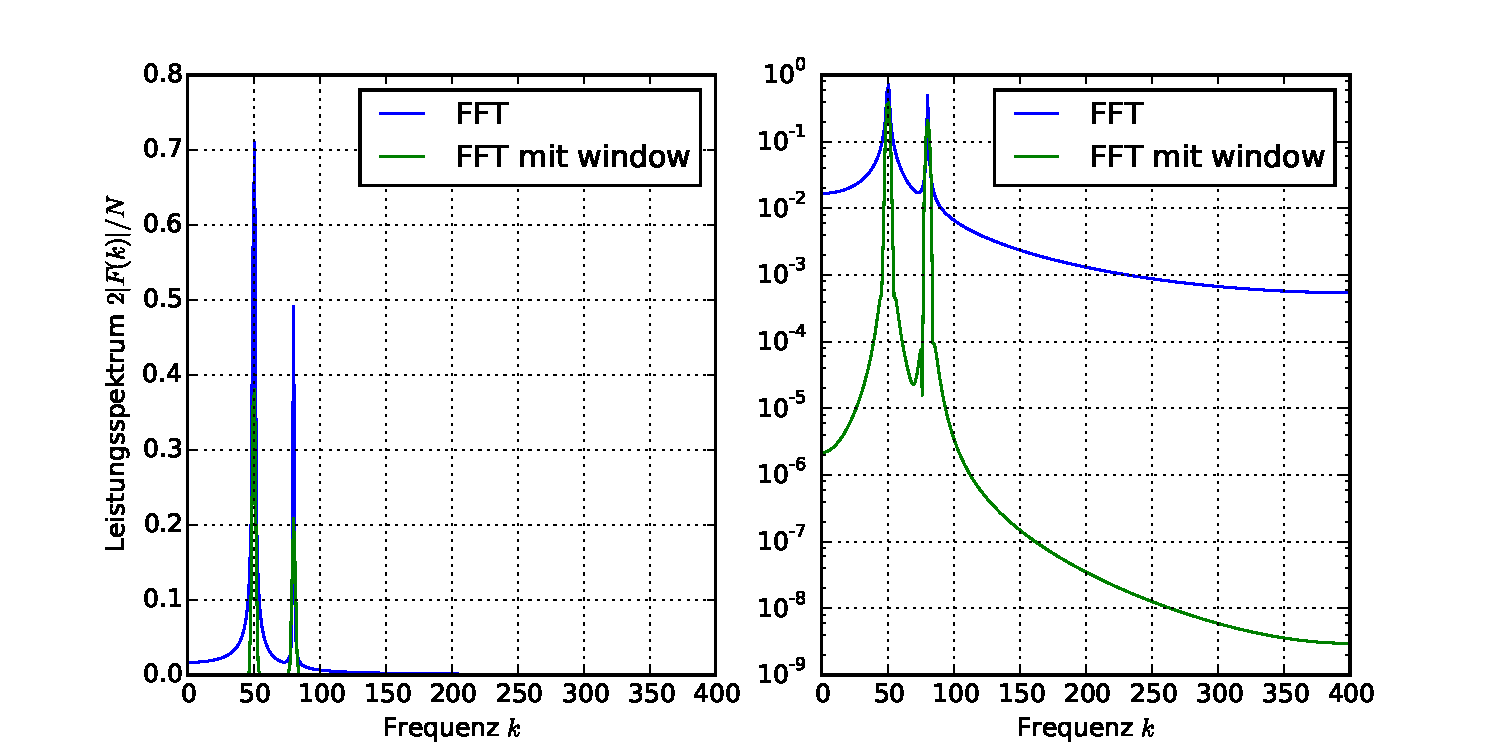
\includegraphics[width=17cm]{pics/stm2}
\caption{Hier berechnen wir numerisch die diskrete
    Fouriertransformation (FFT) des Signals  
$f(t)=\sin(2\pi \omega_1 t) + 0.5 \sin(2\pi \omega_2 t)$ mit den 
Frequenzen $\omega_1 = 50$ und $\omega_2 = 80$, jeweils mit
der Windowfunction \textit{blackman} und ohne. 
Die Berechnung erfolgte mit $N=600$ mithilfe der numerischen
Bibliothek \textit{numpy/scipy} in Python\cite{scipy_reference}.
Der Sourcecode dazu befindet sich im Anhang.
Wie aus den Diagrammen ersichtlich wird, bildet die windowfunktion
\textit{blackman} zusammen mit der FFT
die  beiden Frequenzen $\omega_1$ und $\omega_2$ viel besser ab
als die FFT alleine. Dies ist auch wichtig bei der Analyse der
Datenpunkte aus dem RTM, welche auch nur in diskret vorliegen.
}
 \label{fig:stm2}
\end{figure}


